
%% bare_conf.tex
%% V1.3
%% 2007/01/11
%% by Michael Shell
%% See:
%% http://www.michaelshell.org/
%% for current contact information.
%%
%% This is a skeleton file demonstrating the use of IEEEtran.cls
%% (requires IEEEtran.cls version 1.7 or later) with an IEEE conference paper.
%%
%% Support sites:
%% http://www.michaelshell.org/tex/ieeetran/
%% http://www.ctan.org/tex-archive/macros/latex/contrib/IEEEtran/
%% and
%% http://www.ieee.org/

%%*************************************************************************
%% Legal Notice:
%% This code is offered as-is without any warranty either expressed or
%% implied; without even the implied warranty of MERCHANTABILITY or
%% FITNESS FOR A PARTICULAR PURPOSE! 
%% User assumes all risk.
%% In no event shall IEEE or any contributor to this code be liable for
%% any damages or losses, including, but not limited to, incidental,
%% consequential, or any other damages, resulting from the use or misuse
%% of any information contained here.
%%
%% All comments are the opinions of their respective authors and are not
%% necessarily endorsed by the IEEE.
%%
%% This work is distributed under the LaTeX Project Public License (LPPL)
%% ( http://www.latex-project.org/ ) version 1.3, and may be freely used,
%% distributed and modified. A copy of the LPPL, version 1.3, is included
%% in the base LaTeX documentation of all distributions of LaTeX released
%% 2003/12/01 or later.
%% Retain all contribution notices and credits.
%% ** Modified files should be clearly indicated as such, including  **
%% ** renaming them and changing author support contact information. **
%%
%% File list of work: IEEEtran.cls, IEEEtran_HOWTO.pdf, bare_adv.tex,
%%                    bare_conf.tex, bare_jrnl.tex, bare_jrnl_compsoc.tex
%%*************************************************************************

% *** Authors should verify (and, if needed, correct) their LaTeX system  ***
% *** with the testflow diagnostic prior to trusting their LaTeX platform ***
% *** with production work. IEEE's font choices can trigger bugs that do  ***
% *** not appear when using other class files.                            ***
% The testflow support page is at:
% http://www.michaelshell.org/tex/testflow/



% Note that the a4paper option is mainly intended so that authors in
% countries using A4 can easily print to A4 and see how their papers will
% look in print - the typesetting of the document will not typically be
% affected with changes in paper size (but the bottom and side margins will).
% Use the testflow package mentioned above to verify correct handling of
% both paper sizes by the user's LaTeX system.
%
% Also note that the "draftcls" or "draftclsnofoot", not "draft", option
% should be used if it is desired that the figures are to be displayed in
% draft mode.
%
\documentclass[conference]{IEEEtran}
% Add the compsoc option for Computer Society conferences.
%
% If IEEEtran.cls has not been installed into the LaTeX system files,
% manually specify the path to it like:
% \documentclass[conference]{../sty/IEEEtran}





% Some very useful LaTeX packages include:
% (uncomment the ones you want to load)


% *** MISC UTILITY PACKAGES ***
%
%\usepackage{ifpdf}
% Heiko Oberdiek's ifpdf.sty is very useful if you need conditional
% compilation based on whether the output is pdf or dvi.
% usage:
% \ifpdf
%   % pdf code
% \else
%   % dvi code
% \fi
% The latest version of ifpdf.sty can be obtained from:
% http://www.ctan.org/tex-archive/macros/latex/contrib/oberdiek/
% Also, note that IEEEtran.cls V1.7 and later provides a builtin
% \ifCLASSINFOpdf conditional that works the same way.
% When switching from latex to pdflatex and vice-versa, the compiler may
% have to be run twice to clear warning/error messages.






% *** CITATION PACKAGES ***
%
%\usepackage{cite}
% cite.sty was written by Donald Arseneau
% V1.6 and later of IEEEtran pre-defines the format of the cite.sty package
% \cite{} output to follow that of IEEE. Loading the cite package will
% result in citation numbers being automatically sorted and properly
% "compressed/ranged". e.g., [1], [9], [2], [7], [5], [6] without using
% cite.sty will become [1], [2], [5]--[7], [9] using cite.sty. cite.sty's
% \cite will automatically add leading space, if needed. Use cite.sty's
% noadjust option (cite.sty V3.8 and later) if you want to turn this off.
% cite.sty is already installed on most LaTeX systems. Be sure and use
% version 4.0 (2003-05-27) and later if using hyperref.sty. cite.sty does
% not currently provide for hyperlinked citations.
% The latest version can be obtained at:
% http://www.ctan.org/tex-archive/macros/latex/contrib/cite/
% The documentation is contained in the cite.sty file itself.






% *** GRAPHICS RELATED PACKAGES ***
%
\ifCLASSINFOpdf
  % \usepackage[pdftex]{graphicx}
  % declare the path(s) where your graphic files are
  % \graphicspath{{../pdf/}{../jpeg/}}
  % and their extensions so you won't have to specify these with
  % every instance of \includegraphics
  % \DeclareGraphicsExtensions{.pdf,.jpeg,.png}
\else
  % or other class option (dvipsone, dvipdf, if not using dvips). graphicx
  % will default to the driver specified in the system graphics.cfg if no
  % driver is specified.
  % \usepackage[dvips]{graphicx}
  % declare the path(s) where your graphic files are
  % \graphicspath{{../eps/}}
  % and their extensions so you won't have to specify these with
  % every instance of \includegraphics
  % \DeclareGraphicsExtensions{.eps}
\fi
% graphicx was written by David Carlisle and Sebastian Rahtz. It is
% required if you want graphics, photos, etc. graphicx.sty is already
% installed on most LaTeX systems. The latest version and documentation can
% be obtained at: 
% http://www.ctan.org/tex-archive/macros/latex/required/graphics/
% Another good source of documentation is "Using Imported Graphics in
% LaTeX2e" by Keith Reckdahl which can be found as epslatex.ps or
% epslatex.pdf at: http://www.ctan.org/tex-archive/info/
%
% latex, and pdflatex in dvi mode, support graphics in encapsulated
% postscript (.eps) format. pdflatex in pdf mode supports graphics
% in .pdf, .jpeg, .png and .mps (metapost) formats. Users should ensure
% that all non-photo figures use a vector format (.eps, .pdf, .mps) and
% not a bitmapped formats (.jpeg, .png). IEEE frowns on bitmapped formats
% which can result in "jaggedy"/blurry rendering of lines and letters as
% well as large increases in file sizes.
%
% You can find documentation about the pdfTeX application at:
% http://www.tug.org/applications/pdftex





% *** MATH PACKAGES ***
%
%\usepackage[cmex10]{amsmath}
% A popular package from the American Mathematical Society that provides
% many useful and powerful commands for dealing with mathematics. If using
% it, be sure to load this package with the cmex10 option to ensure that
% only type 1 fonts will utilized at all point sizes. Without this option,
% it is possible that some math symbols, particularly those within
% footnotes, will be rendered in bitmap form which will result in a
% document that can not be IEEE Xplore compliant!
%
% Also, note that the amsmath package sets \interdisplaylinepenalty to 10000
% thus preventing page breaks from occurring within multiline equations. Use:
%\interdisplaylinepenalty=2500
% after loading amsmath to restore such page breaks as IEEEtran.cls normally
% does. amsmath.sty is already installed on most LaTeX systems. The latest
% version and documentation can be obtained at:
% http://www.ctan.org/tex-archive/macros/latex/required/amslatex/math/





% *** SPECIALIZED LIST PACKAGES ***
%
%\usepackage{algorithmic}
% algorithmic.sty was written by Peter Williams and Rogerio Brito.
% This package provides an algorithmic environment fo describing algorithms.
% You can use the algorithmic environment in-text or within a figure
% environment to provide for a floating algorithm. Do NOT use the algorithm
% floating environment provided by algorithm.sty (by the same authors) or
% algorithm2e.sty (by Christophe Fiorio) as IEEE does not use dedicated
% algorithm float types and packages that provide these will not provide
% correct IEEE style captions. The latest version and documentation of
% algorithmic.sty can be obtained at:
% http://www.ctan.org/tex-archive/macros/latex/contrib/algorithms/
% There is also a support site at:
% http://algorithms.berlios.de/index.html
% Also of interest may be the (relatively newer and more customizable)
% algorithmicx.sty package by Szasz Janos:
% http://www.ctan.org/tex-archive/macros/latex/contrib/algorithmicx/




% *** ALIGNMENT PACKAGES ***
%
%\usepackage{array}
% Frank Mittelbach's and David Carlisle's array.sty patches and improves
% the standard LaTeX2e array and tabular environments to provide better
% appearance and additional user controls. As the default LaTeX2e table
% generation code is lacking to the point of almost being broken with
% respect to the quality of the end results, all users are strongly
% advised to use an enhanced (at the very least that provided by array.sty)
% set of table tools. array.sty is already installed on most systems. The
% latest version and documentation can be obtained at:
% http://www.ctan.org/tex-archive/macros/latex/required/tools/


%\usepackage{mdwmath}
%\usepackage{mdwtab}
% Also highly recommended is Mark Wooding's extremely powerful MDW tools,
% especially mdwmath.sty and mdwtab.sty which are used to format equations
% and tables, respectively. The MDWtools set is already installed on most
% LaTeX systems. The lastest version and documentation is available at:
% http://www.ctan.org/tex-archive/macros/latex/contrib/mdwtools/


% IEEEtran contains the IEEEeqnarray family of commands that can be used to
% generate multiline equations as well as matrices, tables, etc., of high
% quality.


%\usepackage{eqparbox}
% Also of notable interest is Scott Pakin's eqparbox package for creating
% (automatically sized) equal width boxes - aka "natural width parboxes".
% Available at:
% http://www.ctan.org/tex-archive/macros/latex/contrib/eqparbox/





% *** SUBFIGURE PACKAGES ***
%\usepackage[tight,footnotesize]{subfigure}
\usepackage{subcaption}
% subfigure.sty was written by Steven Douglas Cochran. This package makes it
% easy to put subfigures in your figures. e.g., "Figure 1a and 1b". For IEEE
% work, it is a good idea to load it with the tight package option to reduce
% the amount of white space around the subfigures. subfigure.sty is already
% installed on most LaTeX systems. The latest version and documentation can
% be obtained at:
% http://www.ctan.org/tex-archive/obsolete/macros/latex/contrib/subfigure/
% subfigure.sty has been superceeded by subfig.sty.


\usepackage{caption}
%\usepackage[caption=false]{caption}
%\usepackage[font=footnotesize]{subfig}
% subfig.sty, also written by Steven Douglas Cochran, is the modern
% replacement for subfigure.sty. However, subfig.sty requires and
% automatically loads Axel Sommerfeldt's caption.sty which will override
% IEEEtran.cls handling of captions and this will result in nonIEEE style
% figure/table captions. To prevent this problem, be sure and preload
% caption.sty with its "caption=false" package option. This is will preserve
% IEEEtran.cls handing of captions. Version 1.3 (2005/06/28) and later 
% (recommended due to many improvements over 1.2) of subfig.sty supports
% the caption=false option directly:
%\usepackage[caption=false,font=footnotesize]{subfig}
%
% The latest version and documentation can be obtained at:
% http://www.ctan.org/tex-archive/macros/latex/contrib/subfig/
% The latest version and documentation of caption.sty can be obtained at:
% http://www.ctan.org/tex-archive/macros/latex/contrib/caption/




% *** FLOAT PACKAGES ***
%
%\usepackage{fixltx2e}
% fixltx2e, the successor to the earlier fix2col.sty, was written by
% Frank Mittelbach and David Carlisle. This package corrects a few problems
% in the LaTeX2e kernel, the most notable of which is that in current
% LaTeX2e releases, the ordering of single and double column floats is not
% guaranteed to be preserved. Thus, an unpatched LaTeX2e can allow a
% single column figure to be placed prior to an earlier double column
% figure. The latest version and documentation can be found at:
% http://www.ctan.org/tex-archive/macros/latex/base/



%\usepackage{stfloats}
% stfloats.sty was written by Sigitas Tolusis. This package gives LaTeX2e
% the ability to do double column floats at the bottom of the page as well
% as the top. (e.g., "\begin{figure*}[!b]" is not normally possible in
% LaTeX2e). It also provides a command:
%\fnbelowfloat
% to enable the placement of footnotes below bottom floats (the standard
% LaTeX2e kernel puts them above bottom floats). This is an invasive package
% which rewrites many portions of the LaTeX2e float routines. It may not work
% with other packages that modify the LaTeX2e float routines. The latest
% version and documentation can be obtained at:
% http://www.ctan.org/tex-archive/macros/latex/contrib/sttools/
% Documentation is contained in the stfloats.sty comments as well as in the
% presfull.pdf file. Do not use the stfloats baselinefloat ability as IEEE
% does not allow \baselineskip to stretch. Authors submitting work to the
% IEEE should note that IEEE rarely uses double column equations and
% that authors should try to avoid such use. Do not be tempted to use the
% cuted.sty or midfloat.sty packages (also by Sigitas Tolusis) as IEEE does
% not format its papers in such ways.





% *** PDF, URL AND HYPERLINK PACKAGES ***
%
%\usepackage{url}
% url.sty was written by Donald Arseneau. It provides better support for
% handling and breaking URLs. url.sty is already installed on most LaTeX
% systems. The latest version can be obtained at:
% http://www.ctan.org/tex-archive/macros/latex/contrib/misc/
% Read the url.sty source comments for usage information. Basically,
% \url{my_url_here}.





% *** Do not adjust lengths that control margins, column widths, etc. ***
% *** Do not use packages that alter fonts (such as pslatex).         ***
% There should be no need to do such things with IEEEtran.cls V1.6 and later.
% (Unless specifically asked to do so by the journal or conference you plan
% to submit to, of course. )


% correct bad hyphenation here
\hyphenation{op-tical net-works semi-conduc-tor}
\usepackage{amsmath,amssymb,graphicx}
\usepackage{tablefootnote}
\usepackage{textcomp}
\makeatletter
\setlength{\@fptop}{0pt}
\makeatother
\setlength{\textfloatsep}{4pt}
\begin{document}
%
% paper title
% can use linebreaks \\ within to get better formatting as desired
\title{A Comparison of Antenna Placement Algorithms\vspace{-1.5ex}}

\author{\IEEEauthorblockN{Abhinav Jauhri}
\IEEEauthorblockA{Carnegie Mellon University\\
ajauhri@cmu.edu}}
\maketitle
\begin{abstract}
%\boldmath
Co-location of multiple antenna systems on a single fixed or mobile platform can be challenging due to a variety of factors, such as mutual coupling, individual antenna constraints, multipath, obstructions, and parasitic effects due to the platform. The situation frequently arises where a new communication capability, and hence antenna system, is needed on an existing platform. The problem of placing new antennas requires a long, manual effort in order to complete an antenna placement study. An automated procedure for determining such placements would not only save time, but would be able to optimize the performance of all co-located antenna systems. In this work, we examine a set of stochastic algorithms to determine their effectiveness at finding optimal placements for multiple antennas on a platform. To our knowledge, this is the first study to investigate optimizing multiple antenna placement on a single platform using multiple stochastic algorithms. Of the four algorithms compared on the basis of convergence rates, simulated annealing and evolutionary strategy were found to be most effective in finding optimal placements.
\end{abstract}
% IEEEtran.cls defaults to using nonbold math in the Abstract.
% This preserves the distinction between vectors and scalars. However,
% if the conference you are submitting to favors bold math in the abstract,
% then you can use LaTeX's standard command \boldmath at the very start
% of the abstract to achieve this. Many IEEE journals/conferences frown on
% math in the abstract anyway.

% no keywords




% For peer review papers, you can put extra information on the cover
% page as needed:
% \ifCLASSOPTIONpeerreview
% \begin{center} \bfseries EDICS Category: 3-BBND \end{center}
% \fi
%
% For peerreview papers, this IEEEtran command inserts a page break and
% creates the second title. It will be ignored for other modes.
\IEEEpeerreviewmaketitle



\section{Introduction}
Antenna placement on a multi-antenna platform currently involves a manual process that is challenging, time consuming, and may result in sub-optimal placements leading to lowered communication systems' performance. Moreover, the search space is highly complex and becomes exponentially large with regard to the number of antennas to be placed ($|\text{search space}| = m^n$, where $m$ is the number of allowable placements for each antenna and $n$ is number of antennas). 

Stochastic optimization techniques have been used extensively for non-convex and nonlinear search spaces to avoid sub-optimal results due to multimodal nature of the search space (see Figure \ref{fig:tc1_ss}). Applying Evolutionary algorithms (EA), a type of stochastic optimization technique, to the antenna placement problem could greatly improve determining acceptable antenna placements. Evolutionary algorithms encompass a variety of computer search technologies, with the Genetic Algorithm (GA) being the most well-known. Moreover, EAs have proven very capable in discovering high performance antenna designs deployed in space \cite{lohn2005evolutionary}. 

In this work, we have analyzed stochastic algorithms to help determine optimal or near-optimal antenna placements on a platform. The problems have been modeled and simulated using antenna modeling software package called NEC2. The approach is agnostic to specifications of the antenna, and the platform. The algorithmic-set include Genetic Algorithm, Evolutionary Strategy, Simulated Annealing, and Hill Climbing.

\section{Related Work}
\label{sec:related}
The problem of optimizing the placement of multiple antennas on a single platform has rarely been studied, if at all.  The closest research we have found concerns algorithms for locating and configuring infrastructure for cellular wireless networks with the assumption of isotropic radiation pattern. Another related work computes optimal antenna locations restricted to a mobile device. In our work, none of the algorithms discussed have prior information of good antenna placements or type of antennas to be placed on the platform.

The related problem of co-designing antennas for a given platform ({\em in-situ} design) using stochastic algorithms has been investigated in \cite{linden2000wire} with encouraging results. Because antenna placement bears many similarities to antenna design, we believe that such algorithms will prove effective.

\section{Problem Formulation}
\label{sec:problem}
\subsection{Inputs}
\label{sec:inputs}
A platform for placing multiple antennas could vary from a simple rectangular box to an aircraft. Our inputs to an algorithm comprise of a platform and set of antennas each with allowable placements on the platform. Formally, a platform, $P$, in 3-dimensional space with its surface discretized into a regular grid with some spacing consisting of potential antenna placement points. Let $n$ denote the number of antennas to be placed on $P$ such that $n>1$, and $A$ represent the set of antennas: $A = \{A_1, ..., A_n\}$. For each antenna $A_i$, $L_i$ denote the set allowable placement coordinates $\in \mathbb R^3$ on $P$ such that the size of $\mid L_i \mid =m_i$, and $ \forall i, m_i>1$:
\[
L_i = \{(x_{1}, y_{1}, z_{1}), ..., (x_{m_i}, y_{m_i}, z_{m_i})\}
\]
For example, Figure \ref{fig:tc1_figure} has $n=2$ and $m=83$ for each antenna.
\begin{figure}%
    \centering
    \begin{subfigure}{\columnwidth}
        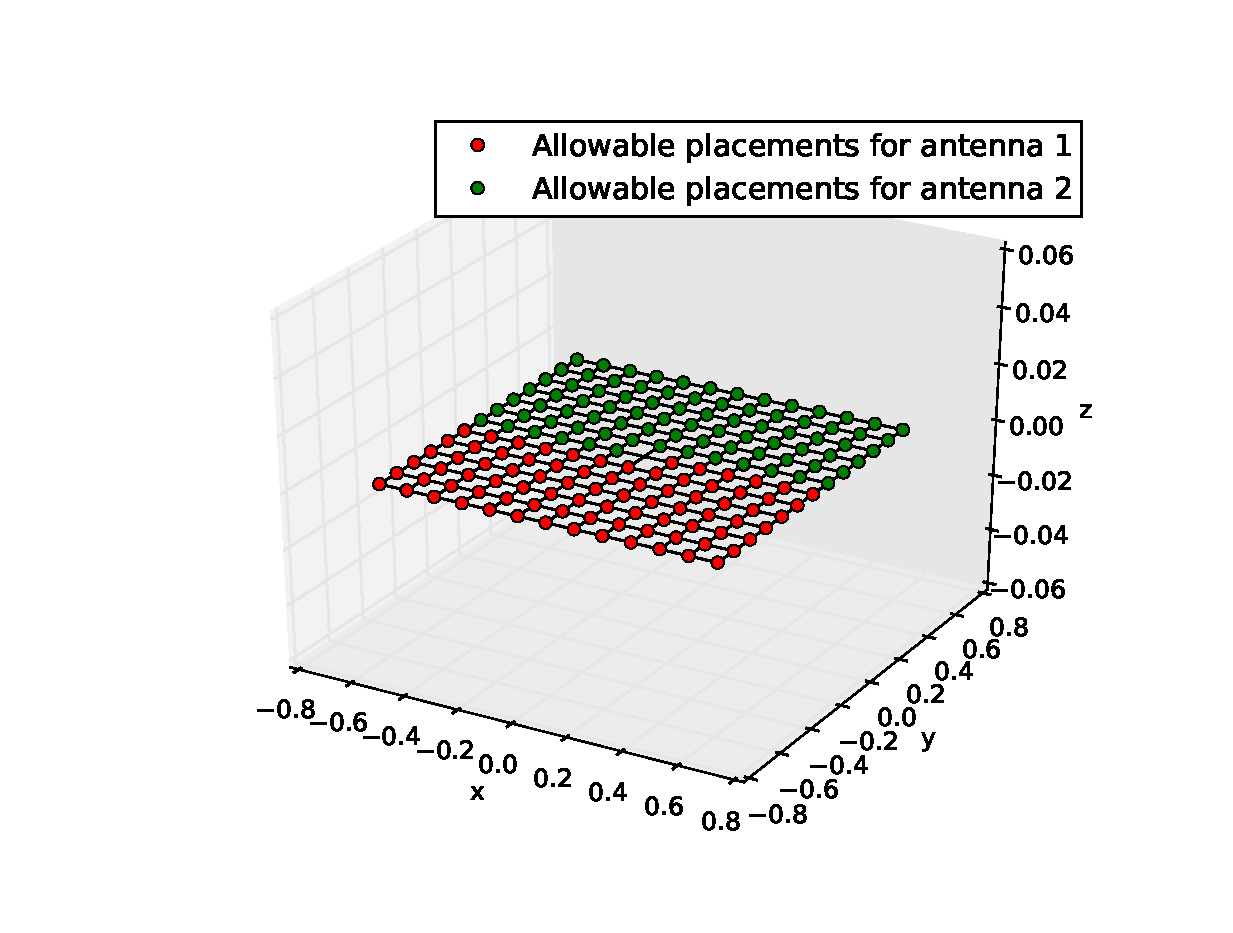
\includegraphics[width=\columnwidth]{FIG/tc_1_figure}%
        \caption{Test Case 1}%
    \label{fig:tc1_figure}%
    \end{subfigure}\hfill%
    \begin{subfigure}{\columnwidth}
        \includegraphics[width=\columnwidth]{FIG/tc1_ss.png}%
        \caption{Search space for test case 1}%
        \label{fig:tc1_ss}%
    \end{subfigure}\hfill\\
\end{figure}


%\begin{figure}
%    \begin{center}
%        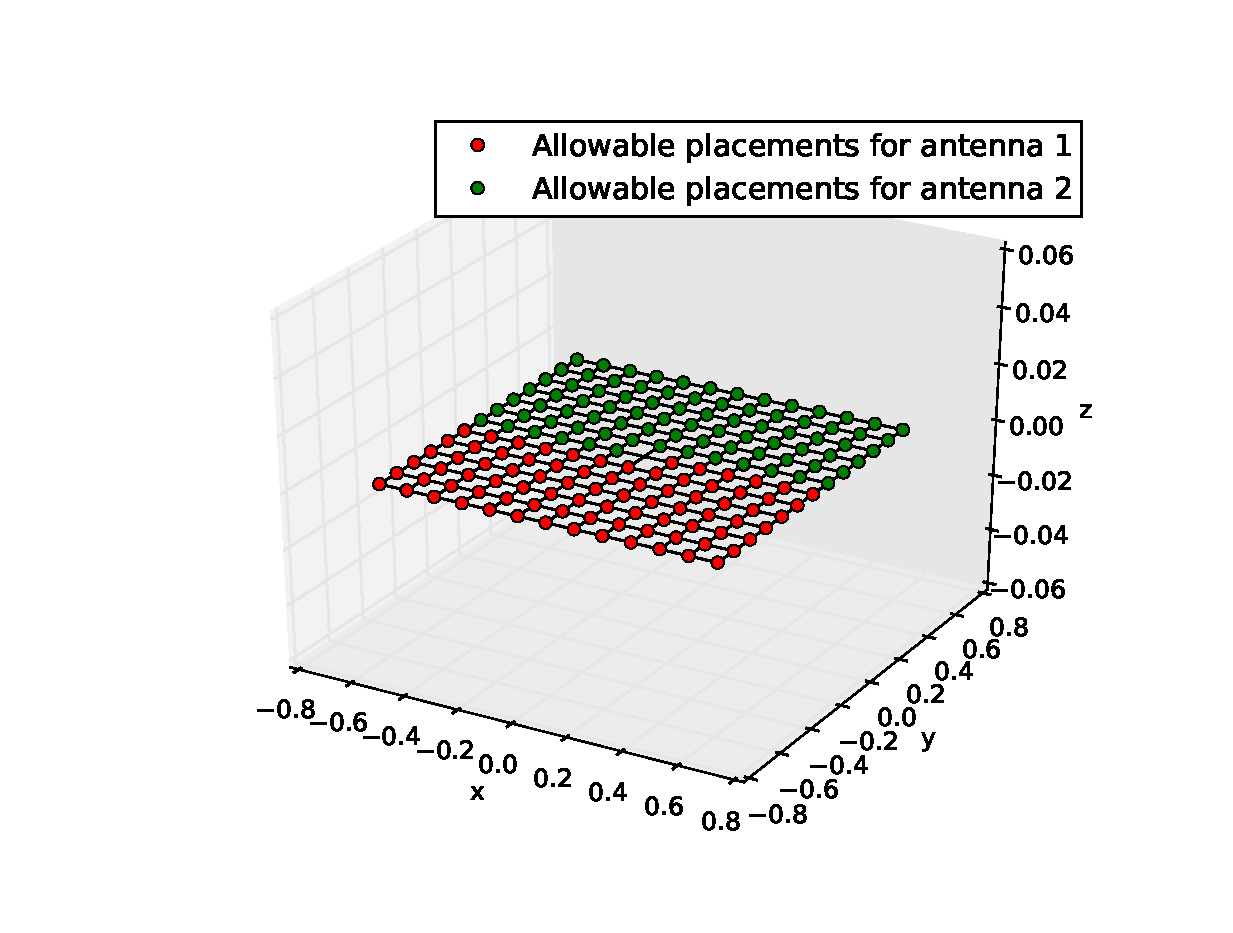
\includegraphics[width=.41\textwidth]{FIG/tc_1_figure}
%\end{center}
%\caption{Test case 1 with two antennas and a square plate. Red dots indicate allowable placements for antenna $1$ and green dots indicate allowable placements for antenna $2$}
%\label{fig:tc1_figure}
%\end{figure}
%
%\begin{figure*}
%    \begin{center}
        %\includegraphics[width=.41\textwidth]{FIG/tc1_ss.png}
%\end{center}
%\caption{Test Case 2}
%\label{fig:tc1_ss}
%\end{figure*}
Using the allowable placements, $L_i$, a \textit{candidate solution/individual}, is a placement configuration of $n$ antenna locations, one for each of the $n$ antennas, in 3-dimensional space:
\[
    \text{Candidate Solution}  = \left\{l_i | l_i \in L_i, i \in [1,n]\right\}
\]
It is important to note that the number of allowable placements for any antenna are finite and discretized. 

\subsection{Fitness Evaluation}
The placement optimization algorithms aim to find the best candidate solution such that the radiation pattern and mutual coupling are optimal. For optimal radiation pattern, we minimize the difference between the free-space gain pattern (FSG) of each antenna $A_i$, and its pattern when placed on a platform and in the presence of all remaining antennas (in-situ gain, or ISG). Minimizing the difference from the free-space gain pattern will ensure better communication capability. For each antenna $A_i$ we compute multiple field points around an antenna in 3-dimensional space:

\begin{equation} \label{eq:rp}
    F_{RP} = \sum_{i=1}^n\sum_{\theta=0}^\pi\sum_{\phi=0}^{2\pi}
           \left| FSG_i(\theta,\phi) - ISG_i(\theta,\phi) \right| ^2,
\end{equation}
where $\theta$ \& $\phi$ define the spherical coordinates of a field point.

For the second objective, it is desired to minimize the mutual coupling between the antennas for a given placement configuration because strong mutual coupling reduces antenna efficiency. This is computed in a pairwise manner where the $CP$ function computes the coupling between two antennas:
\begin{equation}
  F_{MC} = \sum_{i=1}^{n-1}\sum_{j=i+1}^{n} CP(A_i, A_j)
\end{equation}

The overall objective for a given placement configuration is to minimize fitness, $F$:
\begin{equation} \label{eq:optimal}
  F = \alpha F_{MC} + \beta F_{RP},
\end{equation}
where $\alpha$ and $\beta$ are constants such that $\alpha + \beta = 1$.

Radiation pattern and antenna coupling are measured in decibels (dB) which is a logarithmic unit used to express the ratio between two quantities. For radiation pattern parameter, the \textit{antenna strength} or gain shown in Eq.\eqref{eq:rp}, at any given point on a sphere is the ratio of the signal strength of the antenna being tested to a perfectly isotropic antenna. For coupling, the ratio compares the energy absorbed by an antenna when the another antenna is operating nearby. Coupling reduces the antenna's efficiency, and undesirable for the multiple antenna placement problem.

\section{Stochastic Search Algorithms}
\label{sec:algorithms}
%\begin{itemize}
%    \item A hypothesis used by any algorithm is similar to as defined in the previous Section \ref{sec:inputs}.
%    \item For any hypothesis, no two antenna placements overlap. It may be the case that two different antennas have overlapping set of allowable placements, but the formation of any hypothesis avoids such a case as it may result in imprecise calculation of fitness.
%    \item The $fitness(H)$ function used in all four algorithms is the equivalent of Eq.\eqref{eq:optimal}, assuming we have its inputs i.e. $F_{MC}$ and $F_{RP}$.
%\end{itemize}
\subsection{Genetic Algorithm}
\label{sec:algorithms-ga}
Genetic Algorithm aims to model different DNA operations in nature like crossover and mutation. They have been used extensively as stochastic search procedures for numerous applications \cite{fogel1994}.

Operators in our version of GA are \textit{one-point crossover} and \textit{mutation}. Each pair used for one-point crossover operation comprises of an individual uniformly selected from the population and the other from a tournament selection. For all experiments, crossover probability was $60\%$ and mutation probability as $10\%$. Intuitively, a high mutation rate drives the algorithm into a random search and renders evolutionary aspect of the algorithm weak. The size of the individual is not arbitrarily large, and therefore it was preferred to keep the mutation restricted to just manipulating one antenna placement. Since we have a discrete set of placements (end points of wires of a platform), \textit{mutation's} step size involves a new placement from the set of allowable placements for the antenna. This mutation operator is applied to all other algorithms as well.

For arbitrarily large number of antennas, one may need to consider changing the mutation operator to manipulate more than one antenna placement. 
\subsection{Evolutionary Strategy}
\label{sec:algorithms-es}
The evolutionary strategy $(\mu + \lambda)$ is different from a genetic algorithm in the following ways: 
mutation is the primary operator here for maintaining diversity in the population since there are no crossover operations. Survivor selection is done by selecting only fittest $\mu$ individuals to the next generation. A $1/7$ ratio was maintained between $\mu$ and $\lambda$. 

For mutation, both the antenna and its new placement are selected uniformly at random from the allowable placements while ensuring there is no overlap with any other antenna. \textit{Mutation} operator is surely applied once on an individual to generate the offspring.
\subsection{Simulated Annealing}
\label{sec:algoriths-sa}
Simulated annealing models thermodynamics by including a temperature cooling schedule such that it can accept fitness worsening mutation steps with a probability given by Boltzmann distribution. We used a linear cooling schedule for temperature $T_i = \tau T_{i-1}$ with $\tau = f(m_{iters})$. Due to different sizes of the search space, cooling schedule is a function of the maximum iterations ($m_iters$), which are approximately $50\%$ of the total allowable placements. The initial temperature ranged $\in [0.23, 0.27]$.
\subsection{Hill-Climbing}
\label{sec:algoriths-hc}
Hill climbing is a greedy search algorithm different from a simulated annealing since there is no cooling schedule. This makes a hill-climbing prone to get stuck in local optimal solutions. However, the ease of implementation and effectiveness in numerous optimization problems \cite{skalak1994} makes hill-climbing a popular approach.

\section{Experimental Setup}
\label{sec:setup}
We used an open source antenna modeling software called Numerical Electromagnetic Code (NEC2) to calculate the fitness of an individual. NEC2 provides a convenient interface to input details about platform with antennas mounted, and to collect simulation results.

For our experiments, the candidate solution is written to an input file (to be referred as $N_{in}$) which is used by NEC2 modeler to generate an output file (to be referred as $N_{out}$). The platform and all antennas of a candidate solution are written to $N_{in}$ as a set of wires with a start-point and an end-point in 3-dimensional space.  

Figure \ref{fig:plat2} shows the meshed platform depicting a squared plate with box and a sloped front used in test case 2 of our experiments. A square plate with box and sides fixed was the platform for test case 3. For test case 4, the platform was a squared plate as in test case 1 but with four antennas. Possible antenna locations, for all test cases, are defined by either start-points or end-points of platform wires.  
\begin{figure}
    \begin{center}
        \includegraphics[width=.41\textwidth]{FIG/tc_2_figure}
\end{center}
\caption{Test Case 2 with three antennas}
\label{fig:plat2}
\end{figure}

The number of field points in a radiation pattern is determined by the product of total number of unique $\theta$ and $\phi$ values which encompass points in a sphere. All experiments computed the radiation gain over $4140$ points with stepping size being $4$\textdegree $~$ for $\theta$ and $\phi$.

For our placement study, $n$ input files would be generated for a candidate solution with $n$ antennas and only one of the $n$ antennas excited in each input file. Subsequently, NEC2 would generate $n$ output files with performance measures. By exciting one antenna in each input file, we are able to quantify the radiation pattern of an antenna in presence of the platform and other antennas. To determine the free-space gain pattern (FSG) for an antenna, an input file is formed with just the antenna and no platform. $F_{RP}$ is then calculated by \textit{EAP} parsing $2n$ ($n$ files with platform and antennas; $n$ files for free space pattern) output files generated by NEC2.

The second fitness parameter - mutual coupling, is gathered by using $(n+1)th$ file generated. NEC2 generates an output file with mutual coupling results between all possible pairs of antenna placements. If $n=4$, then there are $\binom{4}{2}$ pairs. All test cases were subjected to the same frequency of $100$ MegaHertz.

\begin{table}
\centering
\caption{Antenna Placement Test Cases} \label{tab:tcs}
\begin{tabular}{|c|c|c|} \hline
    Test Case&Number of Antennas&Number of allowable placements\tablefootnote{Allowable placements for each antenna are provided within parenthesis}\\ \hline
1 & 2 & 7,056 (83x83) \\ \hline
2 & 3 & 50,625 (45x45x25) \\ \hline
3 & 3 & 126,025 (71x71x25) \\ \hline
4 & 4 & 20,736 (12x12x12x12) \\
\hline\end{tabular}
\end{table}

\section{Simulation Results}
\label{sec:results}
Comparative study of algorithms is based on multiple test cases listed in Table \ref{tab:tcs}. Each test case was first evaluated with an exhaustive search to determine fitness for all allowable placements of each antenna. The results from exhaustive search were also used to normalize fitness function values between $[0,1]$. For all experiments $\alpha = \beta = 0.5$ in Eq.\eqref{eq:optimal}. 

Genetic Algorithm (GA) and Evolutionary Strategy (ES) operate on a population of candidate solutions at any given time as oppose to Simulated Annealing (SA) and Hill Climber (HC) which operate on one candidate solution. For this reason the mean best fitness in all Figures \ref{fig:tc1_mf}, \ref{fig:tc2_mf}, \ref{fig:tc3_mf}, \& \ref{fig:tc4_mf} is higher in the initial stages of a run for SA/HC than GA/ES. In terms of computational time of any algorithm, the bottleneck is the NEC2 simulator. Therefore, the mean best fitness is shown against the percentage of fitness evaluations which is equivalent to the number of runs of NEC2 simulator. In all four test cases, the best candidate solution was found in less than $25\%$ fitness evaluations of the search space. The termination criteria was either when the global minimum is reached or algorithm evaluates the fitness $0.5 \cdot \left|S\right|$, where $\left|S\right|$ is the size of the search space.

Regions in the plot where the mean best fitness of GA/ES is constant relates to the fitness evaluation of offsprings created by mutation and crossover operators applied on the population. For SA and HC, we notice the SA curve crossing the HC curve in all four test cases. This is due temperature parameter of the SA allowing it to accept fitness worsening individuals with high probability initially in the run. However, later in the run the cooling schedule allows SA to reach a more optimal candidate solution in comparison to the HC.

As known in general, the HC algorithm made progress only in the initial phases of the run and got stuck in local optimums. The purpose for inclusion of such a random search algorithm was to highlight that antenna placements may not always be a trivial optimization task. In test case $4$, the search landscape always has a lower fitness candidate solution in the neighbourhood, therefore allowing HC to converge quickly.

\begin{figure*}%
    \centering
    \begin{subfigure}{\columnwidth}
        \includegraphics[width=\columnwidth]{FIG/tc1_mf.eps}%
        \caption{Test Case 1}%
    \label{fig:tc1_mf}%
    \end{subfigure}\hfill%
    \begin{subfigure}{\columnwidth}
        \includegraphics[width=\columnwidth]{FIG/tc2_mf.eps}%
        \caption{Test Case 2}%
        \label{fig:tc2_mf}%
    \end{subfigure}\hfill\\
    \begin{subfigure}{\columnwidth}
        \includegraphics[width=\columnwidth]{FIG/tc3_mf.eps}%
        \caption{Test Case 3}%
        \label{fig:tc3_mf}%
    \end{subfigure}\hfill%
    \begin{subfigure}{\columnwidth}
        \includegraphics[width=\columnwidth]{FIG/tc4_mf.eps}%
        \caption{Test Case 4}%
        \label{fig:tc4_mf}%
    \end{subfigure}\hfill%
    \caption{Mean best fitness shown for $10$ runs of each algorithm for all test cases. Global minimum calculated using exhaustive search algorithm for each test case shown in magenta on the y-axis. The x-axis is representative of the percentage of fitness evaluations of the search space. They may not be unique points in the search space.}
\end{figure*}
 

\section{Conclusion}
A comparison of four stochastic search algorithms applied to antenna placement optimization was presented. The results showed that a trade-off space exists: faster, less successful Simulated Annealing search versus slower, more successful search by Evolutionary Strategy. The other generation-based algorithm Genetic Algorithm is not as effective as Evolutionary Strategy, and also much slower to find the optimal placements. Our methodology can be applied to any type of a platform which otherwise may be time consuming and expensive in case of large objects like satellites, warships, and aircrafts. Also, a random search was studied to ascertain that the antenna placement problem may not be effectively solved by a greedy algorithm.

Most of the stochastic algorithms presented here were elementary. More experiments can be conducted for population based algorithms with different population sizes, and to statistically compare how this may affect the performance of the algorithm. Also, bigger search spaces need to be considered with more number of antennas. Other evolutionary techniques like ALPS, and Differential Evolution algorithm can also be compared for quality and convergence.

\begin{thebibliography}{1}

\bibitem{lohn2005evolutionary}
Lohn, Jason D., et al. \emph{Evolutionary design of a single-wire circularly-polarized x-band antenna for nasa's space technology 5 mission.} Antennas and Propagation Society International Symposium, 2005 IEEE. Vol. 2. IEEE, 2005.

\bibitem{linden2000wire}
Linden, Derek S. "Wire antennas optimized in the presence of satellite structures using genetic algorithms." Aerospace Conference Proceedings, 2000 IEEE. Vol. 5. IEEE, 2000.

\bibitem{fogel1994}
Fogel, David B. "An introduction to simulated evolutionary optimization." Neural Networks, IEEE Transactions on 5.1 (1994): 3-14.

\bibitem{skalak1994}
Skalak, David B. "Prototype and feature selection by sampling and random mutation hill climbing algorithms." Proceedings of the eleventh international conference on machine learning. 1994.
\end{thebibliography}
\end{document}
